\chapter{总线技术}

总线,即一束公用信号线的集合。其定义了各引线的信号、时序、电气和机械特性,为计算机系统内部各部件、各模块间或计算机各系统之间提供了标准的公共信息通路。
总线一般有内部总线、系统总线和外部总线。
       \begin{description}
             \item[内部总线] 是计算机内部各外围芯片与处理器之间的总线,用于芯片一级的互连;
             \item[系统总线]        是微机中各插件板与系统板之间的总线,用于插件板一级的互连;

             \item[外部总线]        则是微机和外部设备之间的总线,微机作为一种设备,通过该总线和其他设备进行信息与数据交换,它用于设备一级的互连。

           \end{description}




\section{内部总线}

\subsection{I$^2$C总线}

\textbf{I$^2$C(Inter-IC)}总线10多年前由Philips公司推出,是近年来在微电子通信控制领域广泛采用的一种新型总线标准。它是同步通信的一种特殊形式,具有接口线少,控制方式简化,器件封装形式小,通信速率较高等优点。在主从通信中,可以有多个I$^2$C总线器件同时接到I$^2$C 总线上,通过地址来识别通信对象。

\subsection{SPI总线}

\textbf{串行外围设备接口SPI(serial peripheral interface)}总线技术是Motorola公司推出的一种同步串行接口。Motorola公司生产的绝大多数MCU (微控制器)都配有SPI硬件接口,如68系列MCU。SPI 总线是一种三线同步总线,因其硬件功能很强,所以,与SPI有关的软件就相当简单,使CPU有更多的时间处理其他事务 。


\section{系统总线}


\subsection{ISA总线}
IBM公司


\begin{itemize}
  \item 1981年推出基于8位机的PC/XT总线,PC总线
  \item 1984年推出基于16位机的PC/AT总线,AT总线
    但从未公开过AT总线的技术规格
\end{itemize}

Intel公司、IEEE和EISA集团联合推出ISA总线,如图\ref{fig_6_01}所示。

\begin{itemize}
  \item 与IBM/AT原装机总线意义相近的ISA(Industry Standard Architecture)总线,即8/16位的“工业标准结构”:数据传输率最高8MB/s, 寻址空间为$2^{24}=16MB$
\end{itemize}

\begin{figure}
  \centering
  % Requires \usepackage{graphicx}
  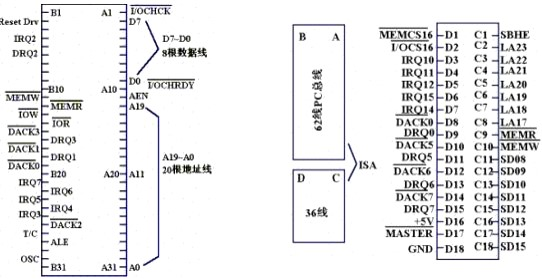
\includegraphics[width=0.6\textwidth]{fig_6_01}\\(a)\\
  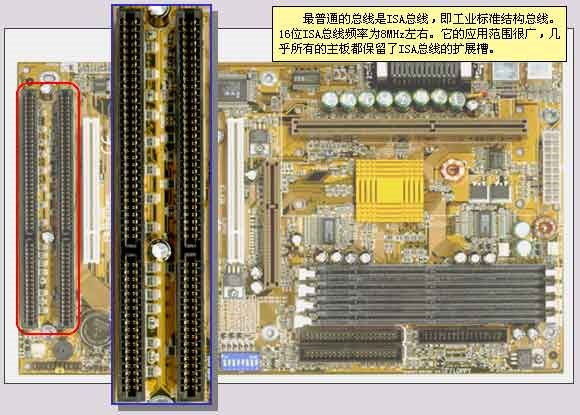
\includegraphics[width=0.4\textwidth]{fig_6_01a}(b)
  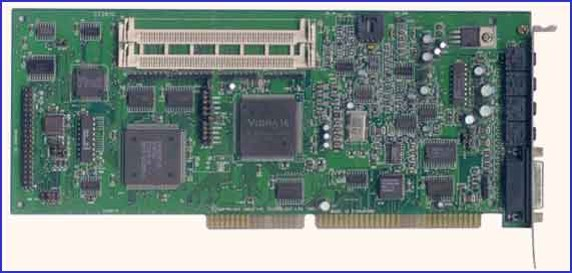
\includegraphics[width=0.4\textwidth]{fig_6_01b}(c)\\
  \caption{ISA总线的IO定义及形式}\label{fig_6_01}
\end{figure}



\subsection{PCI总线}

PCI (Peripheral Component Interconnect)
\begin{itemize}
  \item 现在是主板上最常见的插槽(如下页图示)

  \item 不依附于某个具体的处理器
  \item 结构上是在CPU与原来的系统总线间插入的一级总线,具体由一个桥接电路实现对该层的管理;提供信号缓存,支持10 种外设

  \item 数据总线32/64位,最大传输速率达132MB/s

  \item 可同时支持多组外围设备

\end{itemize}

\begin{figure}
  \centering
  % Requires \usepackage{graphicx}
  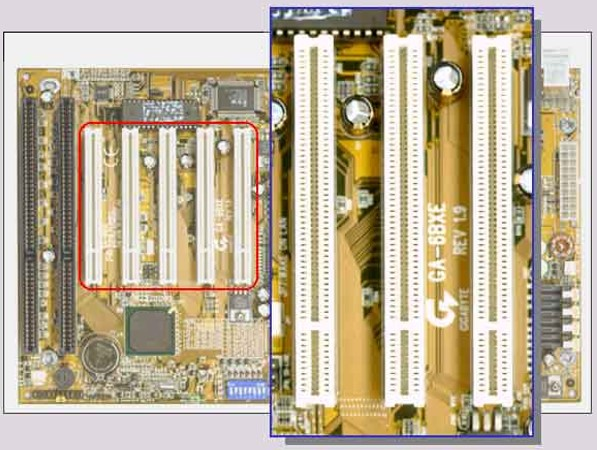
\includegraphics[width=0.3\textwidth]{fig_6_02}(a)
  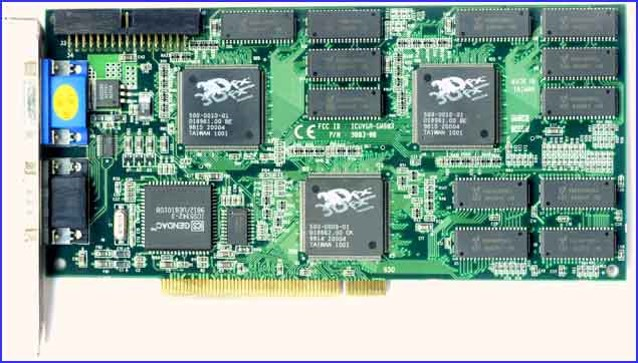
\includegraphics[width=0.4\textwidth]{fig_6_02a}(b)\\
  \caption{PCI总线的形式}\label{fig_6_02}
\end{figure}


\subsection{PC/104总线}


\textbf{PC/104总线}专门为嵌入式控制而定义的工控总线
实质上是一种紧凑型,小型化的 IEEE-P996. 其型号定义和PC/AT基本一致,但电气和机械规范却完全不同,是一种优化的,小型堆栈式结构的嵌入式控制系统。
PC/104总线产品软件上与PC/AT完全兼容。

\subsubsection{PC/104硬件特点:}

\begin{itemize}
  \item 小尺寸结构,标准模块:96x90mm

  \item 堆栈式,“针”“孔”总线连接,即PC/104总线模块之间总线的连接是通过上层的针和下层的孔相互咬和相连,有极好的抗震性。

  \item 4mA总线驱动既可使模块正常工作,低功耗,减少元件数量

  \item 自我堆栈式连接,无须母板

\end{itemize}

\subsubsection{PC/104版本:}
\begin{itemize}
  \item PC/104, 8位,16位分别与PC和PC/AT相对应

  \item PC/104plus则与PCI总线相对应

  \item 一个PC/104 CPU模块则可以同时拥有PC/104和PC/104plus总线

\end{itemize}


\section{外部总线}


\subsection{RS-232-C}

RS—232-C是由美国电子工业协会(EIA)制定的物理接口标准,是RS-232 标准的第3版。是一种应用非常广泛的标准总线,经1987年1月修改后,定名为RS—232-D,但两者差距不大,因此基本成为等同标准。它包括了按位串行传输的电气和机械方面的规定。适合于短距离或带调制解调器的通讯场合。

\begin{enumerate}
  \item 机械指标:标准D型25针插头或9针插头


  \item 电气特性:RS-232-C采用负逻辑,各种信号电平规定如下:

数据信号逻辑“1”:  -3v~-15v(一般用-12v)

数据信号逻辑“0”:  +3v~+15v(一般用十12v)

  \item 通信距离

  RS-232-C标准规定,驱动器可驱动2500pF的电容负载(包括传输介质和接收器输入电容),通信距离将受此电容限制,例如,普通的非屏蔽多芯电缆,每米电容值为131-164pF,因此最大通信距离2500/164≈15m;

\item 信号线定义,如图\ref{fig_6_04}所示。
\begin{figure}
  \centering
  % Requires \usepackage{graphicx}
  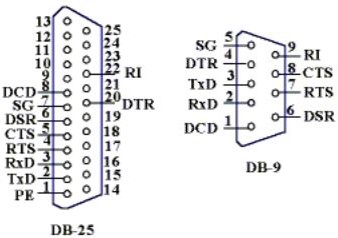
\includegraphics[width=0.3\textwidth]{fig_6_04} (a)
  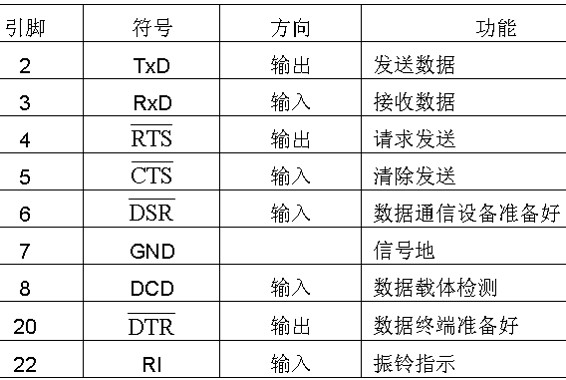
\includegraphics[width=0.3\textwidth]{fig_6_04a} (b)\\
  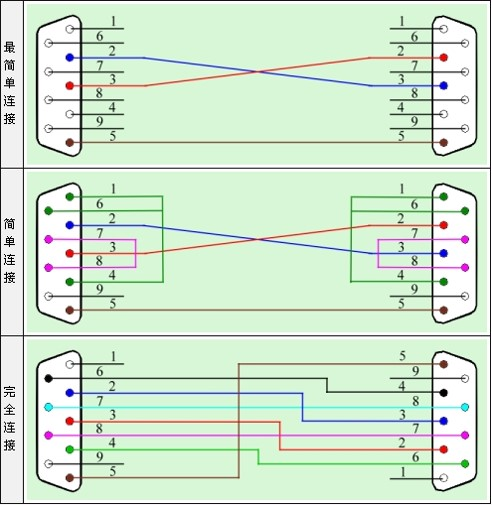
\includegraphics[width=0.3\textwidth]{fig_6_04b} (c)
  \caption{RS-232信号线定义及连接方式}\label{fig_6_04}
\end{figure}

\item 常用芯片: MAX232,MAX202、MAX3232等

\item 连接方式,如图\ref{fig_6_04}(c)所示。



\end{enumerate}




\subsection{RS-485总线}

如图\ref{fig_6_05}所示,RS-485采用平衡差分电路,因此具有抑制共模干扰的能力。加上总线收发器具有高灵敏度,能检测低至200mV的电压,故传输信号能在千米以外得到恢复。

\begin{figure}
  \centering
  % Requires \usepackage{graphicx}
  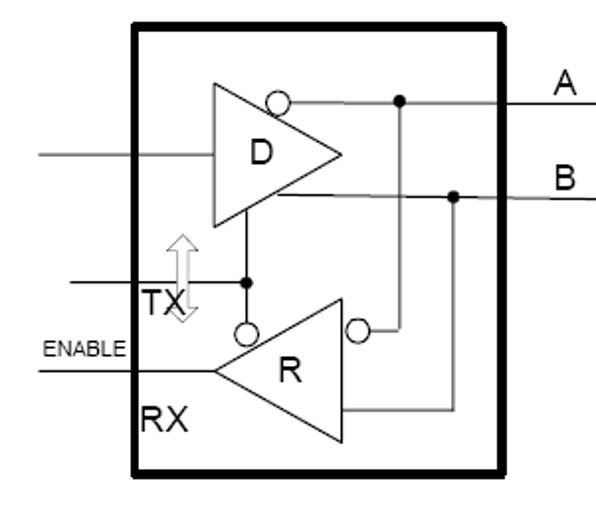
\includegraphics[width=0.24\textwidth]{fig_6_05}(a)
  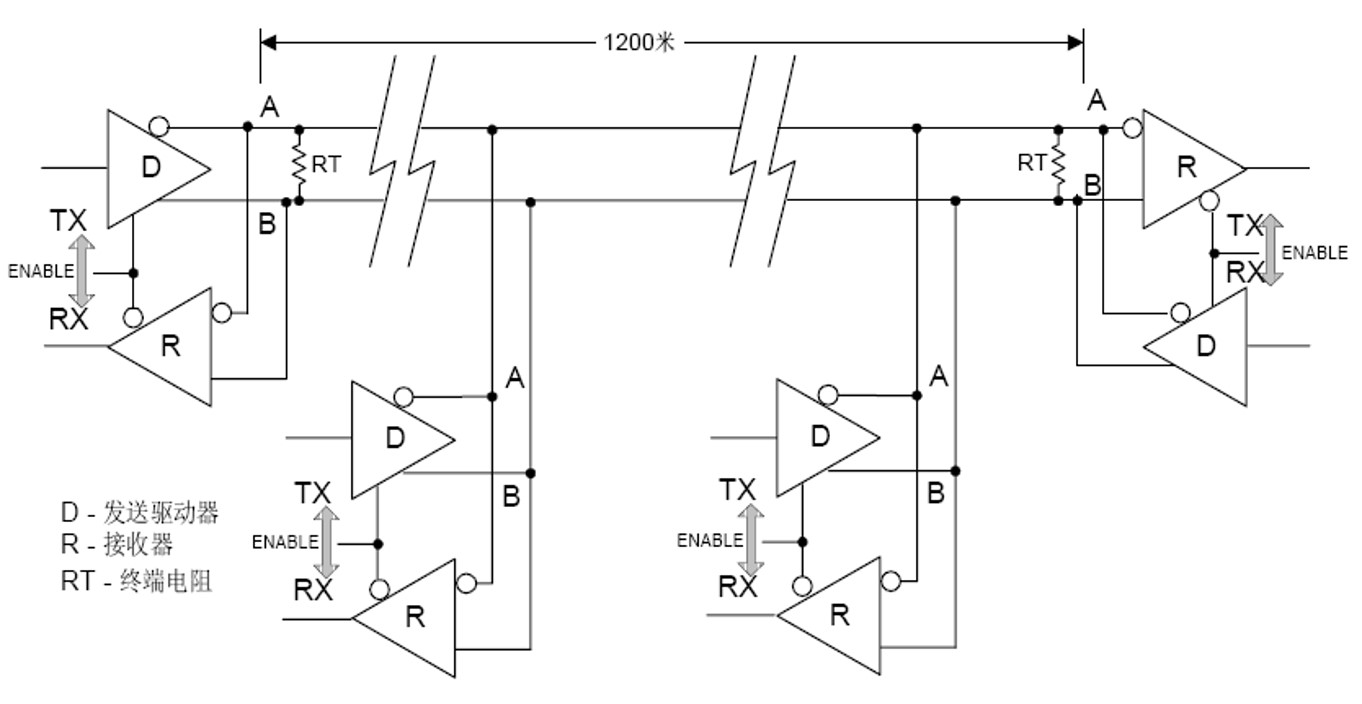
\includegraphics[width=0.4\textwidth]{fig_6_05a}(b)
  \caption{RS-485}\label{fig_6_05}
\end{figure}


\begin{figure}
  \centering
  % Requires \usepackage{graphicx}
  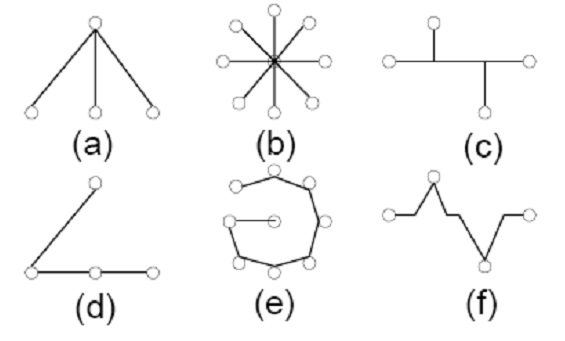
\includegraphics[width=0.4\textwidth]{fig_6_05b}
  \caption{RS-485网络拓扑结构}\label{fig_6_05a}
\end{figure}

如图\ref{fig_6_05a}所示,RS-485 最佳的网络 结构是菊花链形,不要形成很长的支干。其中,(d-f)是好的连接方式。


\begin{remark}

图中\ref{fig_6_05a}(a-c)错误之处在于:信号在各支路末端反射后与原信号迭加,造成信号质量下降。此外,还要注意总线特性阻抗的连续性,在阻抗不连续点也会发生信号的反射。例如,总线的不同区段采用不同电缆或有过长的分支线时都会出线阻抗通信质量严重下降。总之,应该提供一条单一、连续的信号通道作为总线。
\end{remark}


RS-485本身只是物理层的接口规范,只规定了物理接口的机械、电气特性,并没有对通信中的链路连接、网络控制权问题做出相关规定,因而在实际使用中,还需要自定义通信协议或与其它规范中的高层通信协议结合使用(Modbus)。一些现场总线也采用RS -485规范作为其物理层的接口标准,例如:PROFIBUS、BACnet等。


\begin{figure}
  \centering
  % Requires \usepackage{graphicx}
  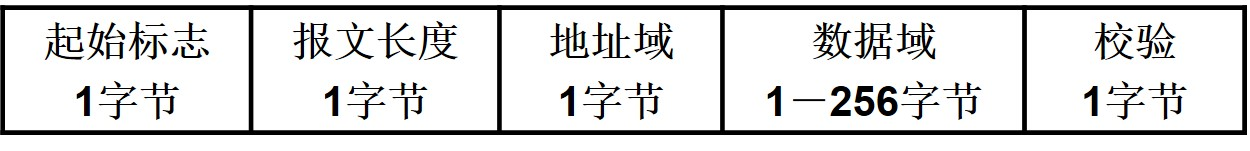
\includegraphics[width=0.4\textwidth]{fig_6_06}
  \caption{RS-485报文内容}\label{fig_6_06}
\end{figure}


\subsection{IEEE-488总线}


IEEE-488是1970年由美国惠普公司开发的并行通讯总线。IEEE-488共定义了24根线(其中8根地线):

\begin{itemize}
  \item
数据总线DIO0~ DIO8
\item 数据传送控制线
\item 数据有效线DAV、未准备好接受数据线NRFD、未接受好数据线NDAC
\item 接口管理总线
\item 接口清除线IFC、服务请求线SQR、注意线ATN、结束或识别线EQI、远程允许REN

\end{itemize}

使用IEEE-488的约定:

\begin{itemize}

\item 数据传输率不得超过每秒1M字节
\item 总线上的设备数不得多于15个
\item 电缆总长度不超过20m,两设备间不超过4m
\item 采用负逻辑


\end{itemize}

\subsection{USB总线}

通用串行总线USB(universal serial bus)是由Intel、 Compaq、Digital、IBM、Microsoft、NEC、Northern Telecom等7家世界著名的计算机和通信公司共同推出的一种新型接口标准。

\begin{itemize}


\item 它基于通用连接技术,实现外设的简单快速连接,达到方便用户、降低成本、扩展PC连接外设范围的目的。
\item 使用新的、通用标准连接器,在计算机上添加设备时不必再打开机箱,安装板卡,甚至都不必重新启动,就可以使用新的设备,USB使您的计算机更易使用。

\item 可以为外设提供电源


\end{itemize}

\begin{itemize}

\item 连结的设备数:
一个USB最多可以连结127个设备

\item 传输速度:


\begin{itemize}
\item 若是使用鼠标或者键盘等不需要高速的设备时,它就采用1.5Mbps的传输速率
\item 若是使用MODEM,音箱、打印机等需要高速传输数据的设备时,则采用12Mbps的同步传输速率(结点间距离5米)。
\item USB2.0标准的MAX传输率480Mbps.


\end{itemize}

\end{itemize}

\subsection{IEEE 1394总线}

IEEE 1394是一种串行接口标准,又名Firewire“火线”,这种接口标准允许把电脑/电脑外部设备/各种家电非常简单地连接在一起。

IEEE 1394的连接电缆中共有六条芯线,其中两条线为电源线,可向被连接的设备提供电源;其它四条线被包装成两对双绞线,用来传输信号,电源的电压范围是8-40V直流电压,最大电流1.5A,像数码相机之类的一些低功耗设备可以从总线电缆内部取得电力,而不必为每一台设备配置独立的供电系统.

1394商业协会正在着手制定IEEE 1394b,这是一个在首阶段会将数据传输速率提高到1.6Gbps、而后计划提高到3.2Gbps的新版本。



\section{现场总线}


变送器、控制器、执行器等现场装置往往采用4-20mA的信号进行通讯联系,无论它们的制造厂商是谁,它们一般都可以互换。从20世纪60年代发展起来的4-20mA信号是一种国际标准,目前仍在使用。
进入20世纪80年代以来,用微处理器技术实现过程控制以及智能传感器的发展导致需要用数字信号取代4-20mA模拟信号,这就形成了现场总线。

\textbf{概念:}国际电工委员会标准IEC61158的定义:现场总线是一种应用于生产现场,在现场设备之间、现场设备与控制装置之间实行双向、串行、多节点数字通信的技术。

一般认为,现场总线是一种全数字化、双向、多站的通信系统,是用于工业控制的计算机系统的工业总线。它是用于生产自动化最底层的现场设备以及现场仪表的互联网络,是现场通信网络和控制系统的集成。

\begin{figure}
  \centering
  % Requires \usepackage{graphicx}
  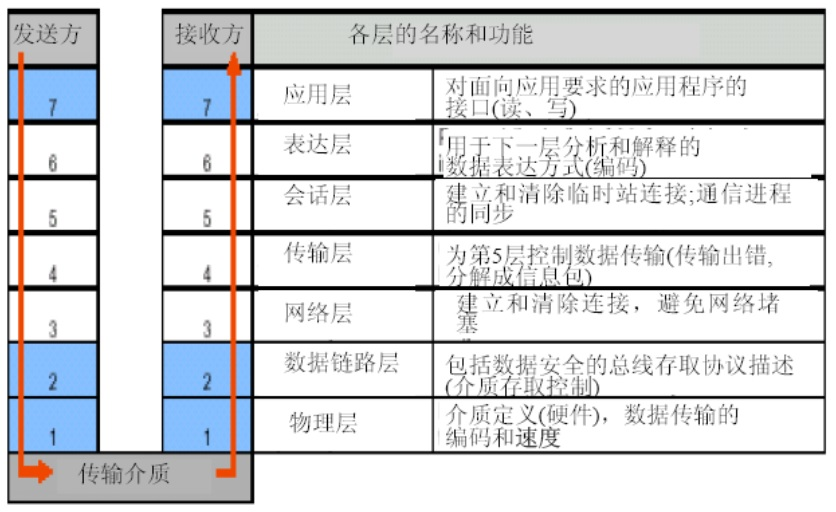
\includegraphics[width=0.6\textwidth]{fig_6_07}
  \caption{OSI参考模型}\label{fig_6_07}
\end{figure}


各厂家在实际制定自己的通信协议时,并非都在产品中实现了这7层协议,而往往依据侧重点的不同,仅仅实现该7层协议的子集。



制订现场总线标准的机构

\begin{itemize}

\item IEC(国际电工委员会)

   IEC/TC65/SC65C/WG6:通过了IEC 61158标准。
   IEC/TC17/SC17B:通过了IEC62026,包括:ASI、DeviceNet、SDS 和Seriplex。


\item ISO(国际标准化组织)
      ISO11898    CAN


\end{itemize}


IEC61158标准的类型:第3版于2003年制定,包括l0种技术类型:

\begin{itemize}

\item 类型1:IEC技术报告(即相当于FF的H1,美国Fisher-Rosemount公司支持);
\item 类型2:ControlNet(美国Rockwell公司支持);
\item 类型3:Profibus(德国Siemens公司支持);
\item 类型4:P-Net(丹麦Process Data公司支持);
\item 类型5:FF HSE(High Speed Ethernet美国Fisher-Rosemount公司支持);
\item 类型6:SwiftNet(美波音公司支持);
\item 类型7:WorldFIP(法国阿尔斯通Alstom公司支持);
\item 类型8:Interbus(德国菲尼克斯Phoenix 公司支持);
\item 类型9:FF应用层(Application Layer);
\item 类型10:Profinet。
\end{itemize}


2007年 ,IEC61158现场总线标准通过,包括20个类型,如图所示。
\begin{figure}
  \centering
  % Requires \usepackage{graphicx}
  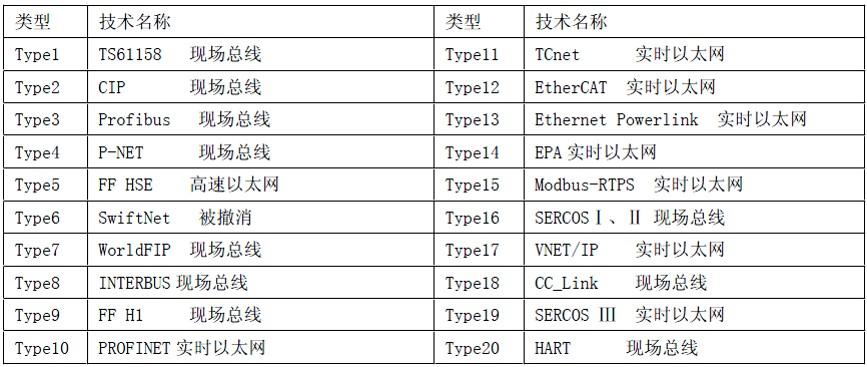
\includegraphics[width=0.6\textwidth]{fig_6_08}
  \caption{现场总线类型}\label{fig_6_08}
\end{figure}




\section{本章要点总结}

\begin{itemize}
  \item 了解各种总线的知识,重点对RS232和RS485进行理解;

  \item 理解现场总线的概念,了解几种典型的现场总线。

\end{itemize}
